\section{\Bash{}}\label{section:bash}

We will preface this section by saying this is by no means the most
comprehensive guide to scripting in \Bash{}. For such a guide, refer to
the official \Bash{} guide here:

\centerline{\url{https://folk.ntnu.no/geirha/bashguide.pdf}}

The amount of \Bash{} knowledge needed for this assignment is very minimal, but
will be crucial to your career in Computer Science. We will start with issuing
commands in \Bash{}.

\subsection{Commands and Arguments}

Commands in \Bash{} are made of up words delimited by whitespace, where a word is
just a sequence of characters. Most commands usually span a single line, but it
is possible to write a more complex line that spans across several lines. As
stated in \S\ref{section:unix}, a command follows the pattern \texttt{command
[arguments]}. Consider the following command:

\begin{shlisting}{}
$ head notes.txt
\end{shlisting}

\Bash{} parses this specific command into two words: \texttt{head} and
\texttt{notes.txt}. The command to execute is \texttt{head} and its sole
argument is \texttt{notes.txt}. The program \texttt{head}, by default, prints
out the first $10$ lines of a specified file, in this case \texttt{notes.txt},
to \emph{standard output}, or \texttt{stdout}. This is what you think of as the
console, or terminal window. Any \Unix{} process has the following three open
input/output streams open at creation:

\begin{enumerate}
  \item Standard input (\texttt{stdin})
  \item Standard output (\texttt{stdout})
  \item Standard error (\texttt{stderr})
\end{enumerate}

What is a \Unix{} process? We'll learn more about that later on in the course,
but for now you can think of it as a program in execution. We'll also discuss
input and output more in-depth later on in this section. Returning back to the
discussion about arguments, it's important to note that there can be any number
of arguments to a command. For instance, the \texttt{head} program also accepts
arguments to specify how many lines of a file to print out. For example, to
print out the first 2 lines of \texttt{notes.txt}:

\begin{shlisting}{}
$ head -n 2 notes.txt
\end{shlisting}

There's not a whole lot more to discuss regarding commands and arguments other
than the different kinds of commands: aliases, functions, built-ins, keywords,
and executables. We will only concern ourselves with built-ins and executables
for now, as they are the bare minimum needed to get moving around in \Unix{} and
writing \Bash{} scripts.

\subsection{Built-ins}

\emph{Built-ins} are functions that are built into \Bash{}. A \Bash{} function
can accept arguments and is composed of a series of commands to execute. For
example, here is a function called \texttt{mkcd} that creates a directory and
enters the created directory:

\begin{shlisting}{}
$ function mkcd { mkdir $1 && cd $1 }
\end{shlisting}

Let's break down this function a bit more. \texttt{mkdir} is a utility that
creates a directory. A directory is the equivalent of a Windows folder. The
\texttt{\$1} accesses the first argument passed to the function. This operates
by parameter expansion (more on this later), as commented in the following
example:

\begin{shlisting}{}
$ mkcd directory # Runs "mkdir directory && cd directory".
\end{shlisting}

The \texttt{\&\&} is a \emph{control operator} and indicates logical AND. So
basically, make the directory with \texttt{mkdir} \emph{and} enter it with
\texttt{cd}. \texttt{cd} is arguably one of the most important built-ins since
its sole purpose is to move around directories. \texttt{echo} is another
built-in.

\subsection{Executables}

An executable on \Unix{} is just another name for a program. The terms
\emph{program}, \emph{executable}, \emph{executable binary}, and sometimes just
\emph{binary}, all refer to a program that can be run, or \emph{executed}. The
distinction between an plain old executable and an executable binary is in its
representation. An executable binary is platform specific and is simply a file
full of machine code: pure binary. An executable could be a shell script, which
contains readable text. The only thing these two share is that they must have
the executable bit set in order to be run. Refer to the discussion of \Unix{}
file permissions in assignment 0 if you have forgotten what the executable bit
refers to.

\subsection{Parameters}

Parameters in \Bash{} store values. There are two kinds of parameters:
\emph{variables} and \emph{special parameters}. Variables are used to store
values specified by the programmer. Special parameters have values that are set
by \Bash{} itself. The value of a parameter can be accessed via \emph{parameter
expansion}, which just means prefixing a parameter's name with a \texttt{\$}. A
parameter name can consist of letters, numbers, and underscores, but cannot
start with a number. An example of \Bash{} variable assignment and parameter
expansion:

\begin{shlisting}{}
$ greeting="Bonjour"
$ prime=13
$ echo $greeting # Prints "Bonjour".
\end{shlisting}

Note that \Bash{} \emph{does not} allow spaces around the assignment operator
due how words are delimited by whitespace. Adding spaces would cause the
assignment to be parsed as three different words instead of one. Special
parameters include \texttt{@} and \texttt{?}, and even \texttt{1} that was used
in an earlier example. Each of these can also be expanded. \texttt{\$@} expands
to all the arguments passed to a command. \texttt{\$?} expands to the exit status
of the last run command. This is typically $0$ for a successful exit, and
non-zero for an unsuccessful exit. \texttt{\$1} expands to the first argument
supplied to a command.

\subsection{Conditionals}

Conditionals allow programming languages to handle decisions and take form as
expressions that can be evaluated as either true or false. \Bash{} uses a
command called \texttt{test} to test whether or not an expression is true. If an
expression is true, \texttt{test} exits with an exit code of 0. Otherwise, it
exits with an exit code of 1. For example:

\begin{shlisting}{}
$ test "hello = hello"
$ echo $? # Prints out last command's exit code, which is 0.
$ test "hello = goodbye"
$ echo $? # Prints 1.
\end{shlisting}

\Bash{}, unlike several programming languages, uses \texttt{=} instead of
\texttt{==} to test for equality. As you may expect, \Bash{} also provides
\texttt{if-else} statements.

\begin{shlisting}{}
$ if [ -f mystery ]; then echo "file"; else echo "directory"; fi
\end{shlisting}

This example tests if \texttt{mystery} is a file. The square brackets indicate a
test (\texttt{[} is a reserved keyword for the \texttt{test} command), and
\texttt{-f} tests if its argument is a file. \Bash{} has a more robust keyword
for testing, \texttt{[[}, which should be preferred over \texttt{[} since it
provides more functionality.

\begin{shlisting}{}
$ if [[ -d mystery ]]; then echo "directory"; else echo "file"; fi
\end{shlisting}

\subsection{Loops}

Loops allow for commands to be executed multiple times in succession. We will
discuss the \texttt{while} and \texttt{for}-loop in \Bash{}, since they also
appear in \textbf{C}. The \texttt{while}-loop loops until a command exits
unsuccessfully.

\begin{shlisting}{}
$ while true; do echo "infinitely looping"; done
\end{shlisting}

There are two \texttt{for}-loop flavors. One of them closely resembles a
\texttt{for}-loop in \C{}.

\begin{shlisting}{}
$ for (( i=0; i < 10; i++ )); do echo $i; done
\end{shlisting}

What is the \texttt{(( ... ))}? That is an \emph{arithmetic context} in \Bash{}.
\Bash{} inherently handles variables as just text. Try the following example:

\begin{shlisting}{}
$ x=3
$ y=29
$ if [[ $x > $y ]]; then echo "x > y"; else echo "x <= y"; fi
\end{shlisting}

Why does it print \texttt{"x > y"}? Because it compared \texttt{x} and
\texttt{y} \emph{lexicographically}. To test things numerically, we need to use
an arithmetic context.

\begin{shlisting}{}
$ x=3
$ y=29
$ if (( $x > $y )); then echo "x > y"; else echo "x <= y"; fi
\end{shlisting}

You can think of an arithmetic context as just an environment in which numerical
operations such as addition and multiplication can be performed. This is needed
for the \texttt{for}-loop because \texttt{++} is the \emph{postfix increment
operator}. You will learn more about the differences between the postfix and
prefix operators when you start writing \C{} programs.

The other \texttt{for}-loop in \Bash{} uses \emph{brace expansion}, like so:

\begin{shlisting}{}
$ for i in {0..9}; do echo $i; done
\end{shlisting}

\Bash{} handles \texttt{\{0..9\}} by expanding it to the list of words \texttt{0
1 2 3 4 5 6 7 8 9}. The variable \texttt{i} is then assigned to each expanded
word in sequence. The \texttt{..} indicates a \emph{range} in \Bash{}. Ranges in
\Bash{} are inclusive.

You can iterate over more than just integers in \Bash{}; you can even iterate
over all the files in the current directory that end in \texttt{.txt}.

\begin{shlisting}{}
$ for f in *.txt; do echo "$f seems like a text file"; done
\end{shlisting}

The \texttt{*} used in the \texttt{for}-loop is a \emph{glob}. Globs are used
for matching patterns. The \texttt{*} glob in particular matches any string.
Thus, \texttt{*.txt} matches any string as long as it ends with \texttt{.txt}.
Globs are very closely related to \emph{regular expressions}, which you'll
become acquainted with later on in the course.

\subsection{Input and Output}

As stated earlier, any \Unix{} process starts up with \texttt{stdin},
\texttt{stdout}, and \texttt{stderr}. We described them as input/output streams
earlier, but that was a slight lie. To be more exact, these are all \emph{file
descriptors}. File descriptors are simply integers that act as indices into a
table of open files for a process. By default, \texttt{stdin} is file descriptor
0, \texttt{stdout} is file descriptor 1, and \texttt{stderr} is file descriptor
2. \texttt{stdin} is where input goes, such as a typed password when a program
prompts for one. \texttt{stdout} and \texttt{stderr} both print to the console,
with the only difference being that \texttt{stderr} is usually designated for
error messages. \Bash{} has two main mechanisms to provide input/output
redirection: \emph{file redirection}, and \emph{pipes}.

\subsubsection{File Redirection}

File redirection works for both input and output. That is, you can specify that
a program take input from a file (redirecting \texttt{stdin}) and place its
output into another file (redirecting \texttt{stdout}).

\begin{shlisting}{}
$ head < full.txt > first10.txt
\end{shlisting}

This example first redirects the \texttt{stdin} of \texttt{head} to
\texttt{full.txt}. In other words, it feeds the contents of \texttt{full.txt} to
\texttt{head}. Then, it then \texttt{stdout} of \texttt{head} is redirected to
\texttt{first10.txt}. This takes the output produced by \texttt{head} and places
it in \texttt{first10.txt}. As you can imagine, \texttt{<} is the input
redirection keyword and \texttt{>} is the output redirection keyword. To
redirect \texttt{stderr}, prefix the output redirect keyword with the file
descriptor of \texttt{stderr}: $2$.

\begin{shlisting}{}
$ head < full.txt > first10.txt 2> errors.txt
\end{shlisting}

We can build on this example further, redirecting \texttt{stdout} to
\texttt{/dev/null}, then redirecting \texttt{stderr} to what \texttt{stdout} is
pointing at. \texttt{/dev/null} can be thought of as a black hole: it consumes
anything that is written to it. Note that \texttt{>} by default redirects
\texttt{stdout}. We could also manually specify to redirect \texttt{stdout} with
\texttt{1>}.

\begin{shlisting}{}
$ head < full.txt > /dev/null 2>&1
\end{shlisting}

\subsubsection{Pipes}

It is with \emph{pipes} where you can truly see and appreciate the beauty of the
\Unix{} philosophy. Pipes, originally called \emph{hoses}, allow for the
\texttt{stdout} of one process to be connected, or piped, to the \texttt{stdin}
of another process.

\begin{shlisting}{}
$ ls | sort -r
\end{shlisting}

This is an example of a \Unix{} \emph{pipeline}: two or more commands piped
together. This particular pipeline lists the contents of the current directory
in reverse lexicographic order. Hopefully it's easy to see why the \Unix{}
philosophy is so loved and still widely used today. Just consider the following
example, which prints out your most commonly used commands and the number of
times you've used the command.

\begin{shlisting}{}
$ history | awk '{ $1=""; print $0 }' | sort | uniq -c | sort -nr
\end{shlisting}

\subsection{Here-Documents}

A \emph{here-document}, or \emph{heredoc}, is another way of passing data into a
command. This is typically used if you don't have too much information to pass
along to a command and don't want to write it to a file first and then redirect
it. We'll use an example of a here-document in the next section when we tackle a
simple script using \texttt{gnuplot}.

\subsection{A Simple \Bash{} Script}

We can now start to write \Bash{} scripts. We'll start with a simple script that
plots the function $\sin(x)$ using values of $x$ within the range $[-2\pi,
2\pi)$ in increments of 0.01. This script is provided as \texttt{plot.sh} in
resource repository. Refer to Figure \ref{figure:sinplot} for what the
produced plot should resemble.

\begin{figure}[htb]
  \centering
  % GNUPLOT: LaTeX picture with Postscript
\begingroup
  \makeatletter
  \providecommand\color[2][]{%
    \GenericError{(gnuplot) \space\space\space\@spaces}{%
      Package color not loaded in conjunction with
      terminal option `colourtext'%
    }{See the gnuplot documentation for explanation.%
    }{Either use 'blacktext' in gnuplot or load the package
      color.sty in LaTeX.}%
    \renewcommand\color[2][]{}%
  }%
  \providecommand\includegraphics[2][]{%
    \GenericError{(gnuplot) \space\space\space\@spaces}{%
      Package graphicx or graphics not loaded%
    }{See the gnuplot documentation for explanation.%
    }{The gnuplot epslatex terminal needs graphicx.sty or graphics.sty.}%
    \renewcommand\includegraphics[2][]{}%
  }%
  \providecommand\rotatebox[2]{#2}%
  \@ifundefined{ifGPcolor}{%
    \newif\ifGPcolor
    \GPcolorfalse
  }{}%
  \@ifundefined{ifGPblacktext}{%
    \newif\ifGPblacktext
    \GPblacktexttrue
  }{}%
  % define a \g@addto@macro without @ in the name:
  \let\gplgaddtomacro\g@addto@macro
  % define empty templates for all commands taking text:
  \gdef\gplbacktext{}%
  \gdef\gplfronttext{}%
  \makeatother
  \ifGPblacktext
    % no textcolor at all
    \def\colorrgb#1{}%
    \def\colorgray#1{}%
  \else
    % gray or color?
    \ifGPcolor
      \def\colorrgb#1{\color[rgb]{#1}}%
      \def\colorgray#1{\color[gray]{#1}}%
      \expandafter\def\csname LTw\endcsname{\color{white}}%
      \expandafter\def\csname LTb\endcsname{\color{black}}%
      \expandafter\def\csname LTa\endcsname{\color{black}}%
      \expandafter\def\csname LT0\endcsname{\color[rgb]{1,0,0}}%
      \expandafter\def\csname LT1\endcsname{\color[rgb]{0,1,0}}%
      \expandafter\def\csname LT2\endcsname{\color[rgb]{0,0,1}}%
      \expandafter\def\csname LT3\endcsname{\color[rgb]{1,0,1}}%
      \expandafter\def\csname LT4\endcsname{\color[rgb]{0,1,1}}%
      \expandafter\def\csname LT5\endcsname{\color[rgb]{1,1,0}}%
      \expandafter\def\csname LT6\endcsname{\color[rgb]{0,0,0}}%
      \expandafter\def\csname LT7\endcsname{\color[rgb]{1,0.3,0}}%
      \expandafter\def\csname LT8\endcsname{\color[rgb]{0.5,0.5,0.5}}%
    \else
      % gray
      \def\colorrgb#1{\color{black}}%
      \def\colorgray#1{\color[gray]{#1}}%
      \expandafter\def\csname LTw\endcsname{\color{white}}%
      \expandafter\def\csname LTb\endcsname{\color{black}}%
      \expandafter\def\csname LTa\endcsname{\color{black}}%
      \expandafter\def\csname LT0\endcsname{\color{black}}%
      \expandafter\def\csname LT1\endcsname{\color{black}}%
      \expandafter\def\csname LT2\endcsname{\color{black}}%
      \expandafter\def\csname LT3\endcsname{\color{black}}%
      \expandafter\def\csname LT4\endcsname{\color{black}}%
      \expandafter\def\csname LT5\endcsname{\color{black}}%
      \expandafter\def\csname LT6\endcsname{\color{black}}%
      \expandafter\def\csname LT7\endcsname{\color{black}}%
      \expandafter\def\csname LT8\endcsname{\color{black}}%
    \fi
  \fi
    \setlength{\unitlength}{0.0500bp}%
    \ifx\gptboxheight\undefined%
      \newlength{\gptboxheight}%
      \newlength{\gptboxwidth}%
      \newsavebox{\gptboxtext}%
    \fi%
    \setlength{\fboxrule}{0.5pt}%
    \setlength{\fboxsep}{1pt}%
    \definecolor{tbcol}{rgb}{1,1,1}%
\begin{picture}(7200.00,5040.00)%
    \gplgaddtomacro\gplbacktext{%
      \csname LTb\endcsname%%
      \put(946,704){\makebox(0,0)[r]{\strut{}$-1$}}%
      \put(946,1072){\makebox(0,0)[r]{\strut{}$-0.8$}}%
      \put(946,1439){\makebox(0,0)[r]{\strut{}$-0.6$}}%
      \put(946,1806){\makebox(0,0)[r]{\strut{}$-0.4$}}%
      \put(946,2174){\makebox(0,0)[r]{\strut{}$-0.2$}}%
      \put(946,2542){\makebox(0,0)[r]{\strut{}$0$}}%
      \put(946,2909){\makebox(0,0)[r]{\strut{}$0.2$}}%
      \put(946,3277){\makebox(0,0)[r]{\strut{}$0.4$}}%
      \put(946,3644){\makebox(0,0)[r]{\strut{}$0.6$}}%
      \put(946,4012){\makebox(0,0)[r]{\strut{}$0.8$}}%
      \put(946,4379){\makebox(0,0)[r]{\strut{}$1$}}%
      \put(1078,484){\makebox(0,0){\strut{}$-8$}}%
      \put(1794,484){\makebox(0,0){\strut{}$-6$}}%
      \put(2509,484){\makebox(0,0){\strut{}$-4$}}%
      \put(3225,484){\makebox(0,0){\strut{}$-2$}}%
      \put(3941,484){\makebox(0,0){\strut{}$0$}}%
      \put(4656,484){\makebox(0,0){\strut{}$2$}}%
      \put(5372,484){\makebox(0,0){\strut{}$4$}}%
      \put(6087,484){\makebox(0,0){\strut{}$6$}}%
      \put(6803,484){\makebox(0,0){\strut{}$8$}}%
    }%
    \gplgaddtomacro\gplfronttext{%
      \csname LTb\endcsname%%
      \put(209,2541){\rotatebox{-270}{\makebox(0,0){\strut{}$y$}}}%
      \put(3940,154){\makebox(0,0){\strut{}$x$}}%
      \csname LTb\endcsname%%
      \put(3940,4709){\makebox(0,0){\strut{}$y = \sin(x)$}}%
    }%
    \gplbacktext
    \put(0,0){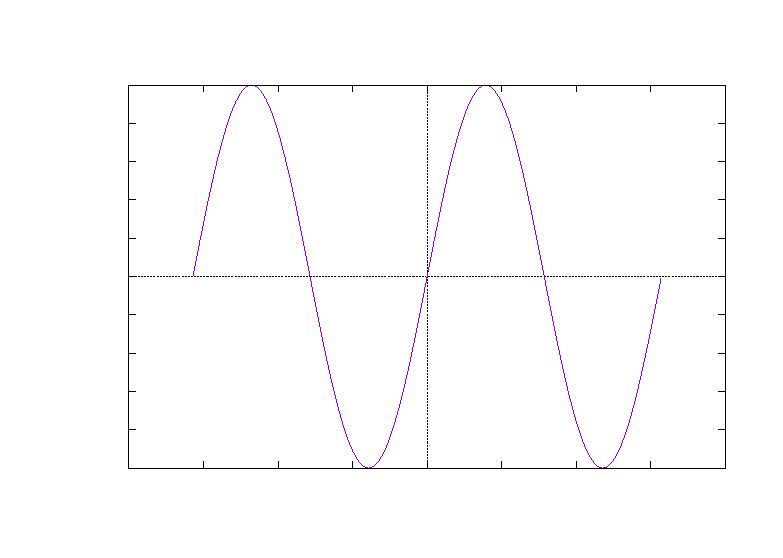
\includegraphics[width={360.00bp},height={252.00bp}]{figures/sinplot}}%
    \gplfronttext
  \end{picture}%
\endgroup

  \caption{\label{figure:sinplot}
    Values of $\sin(x)$ over $x$ in $[-2\pi, 2\pi)$.
  }
\end{figure}

% Use pylisting for nicer colors.
\begin{pylisting}{\texttt{plot.sh}}
#!/bin/bash

make clean && make sincos   # Rebuild the sincos executable.
./sincos > /tmp/sin.dat     # Place the data points into a file.

# This is the here-document that is sent to gnuplot.
gnuplot <<END
    set terminal pdf
    set output "sin.pdf"
    set title "sin(x)"
    set xlabel "x"
    set ylabel "y"
    set zeroaxis
    plot "/tmp/sin.dat" with lines title ""
END
\end{pylisting}

The first line, although it starts with the comment character \texttt{\#}, is
imperative. It acts as the \emph{interpreter directive}. When \texttt{plot.sh}
is executed, the first two bytes of the file, \texttt{\#!}, indicate that
\texttt{plot.sh} is a executable script and the program to use to interpret
the script is \texttt{/bin/bash}. To set the executable bit of
\texttt{plot.sh}, use \texttt{chmod}:

\begin{shlisting}{}
$ chmod +x plot.sh
\end{shlisting}

To run the script:

\begin{shlisting}{}
$ ./plot.sh
\end{shlisting}

The syntax for a here-document may look a little strange. An identifier is
required to delineate the start and end of the here-document. In the case of
\texttt{plot.sh}, the identifier \texttt{END} is used. Any identifier is fine as
long as the contents of the here-document don't also use the identifier. It
should be clear that \texttt{gnuplot} is the intended destination command for
this particular here-document, but here-documents in general can be sent to any
command.
